%!TEX TS-program = xelatex
%!TEX encoding = UTF-8 Unicode

\def \papersize {a4paper}
\documentclass[12pt,\papersize]{extarticle}
% extarticle is like article but can handle 8pt, 9pt, 10pt, 11pt, 12pt, 14pt, 17pt, and 20pt text

\def \ititle {Mindreading and Joint Action: Philosophical Tools}
\def \isubtitle {Notes for Lecture 6}
\def \iauthor {Stephen A. Butterfill}
\def \iemail{ButterfillS@ceu.hu}
%for anonymous submisison
%\def \iauthor {}
%\def \iemail{}
%\date{}

\input{$HOME/Documents/submissions/preamble_steve_paper3}

%avoid overhang
\tolerance=5000


\begin{document}

\setlength\footnotesep{1em}

\bibliographystyle{newapa} %apalike

%these two lines are for anonymous submission --- they remove author and date
%but don't forget to remove defs above as well --- otherwise it will be in the metadata
%\author{}
%\date{}


\maketitle
%\tableofcontents
%
%\begin{abstract}
%\noindent
%***
%\ 
%
%\noindent
%\textbf{Keywords:}
%Mindreading, Joint Action, Action, Belief, Intention, Representation, Mental State
%\end{abstract}
%

\section{***Comments}
1. Csibra.  I completely agree.  I already said this \citep{Csibra:2007fy}.

2. Have to allow for learning new ways of doing things.  Have to allow that I might see an action and come to realise that this is a better way of achieving G than anything I would actually plan.


\section{Goal Ascription}
Purposive action is action directed to the realisation of one or more outcomes.

\newcommand{\dfGoalAscription}{\emph{Goal ascription} is the process of identifying outcomes to which purposive actions are directed as outcomes to which those actions are directed.}

\dfGoalAscription{}


To illustrate, suppose that
Hannah kicks a ball thereby both preventing her sisters from scoring and also breaking a window.
Asked about the episode,
Hannah might protest, truthfully, that the goal of her action was not to break the window but only to reverse the others' advance.
As this illustrates,
among the actual and possible outcomes of an action,
only some are outcomes to which the action is directed.
Goal ascription is the process of identifying 
 those outcomes as outcomes to which the action is directed.


\section{Pure goal ascription}
In this lecture I want us to focus on \emph{pure} goal ascription, that is goal ascription which occurs independently of any knowledge of mental states.

It is quite natural to think that there are primitive kinds of goal ascription which do not require  representing any mental states at all.
Certainly this possibility is assumed  in both developmental and comparative research on goal ascription.%
\footnote{ 
Compare \citet{Gergely:1995sq},
	\citet{Woodward:1998dm} and
	\citet{Penn:2007ey}
among many others.
}
And I also assumed it in the construction of a minimal theory of mind in the second lecture.


The question for this lecture is,
\newcommand{\theQuestion}{How could pure goal ascription work? }
\textbf{\theQuestion} 
How could you identify the goals of an action without ascribing intentions or other mental states to its agent?

Before getting started, I want to step back and first explain why I think we should be excited about pure goal ascription.

Goal ascription enables us to
	predict and manipulate others' actions
	and to learn from their 
		failures 
	as well as their 
		successes.
But there are deeper reasons for excitement.

Pure goal ascription is more primitive than either mindreading or joint action, and both mindreading and joint action depend on it.
Let me explain ...


\subsection{The emergence of social cognition}
Pure goal ascription provides for the possibility of simple forms of joint action,
	which in turn enable us to explain the emergence, in evolution or development, of mindreading and ostensive communication.
In short, having a good account of pure goal ascription is essential for understanding how sophisticated forms of social cognition and communication could emerge.
(This is something I'll explain properly in later lectures.)

\subsection{Epistemic basis of mindreading}
A further motive for asking how pure goal ascription is possible is that it seems to be essential in many cases of mindreading.

To see why we need to step right back for a moment.
\textit{Mindreading} is 
	the process of 
	identifying mental states and actions 
	as the mental states and actions 	of a particular subject 
	on the basis, ultimately, of bodily movements and their absence,
somewhat as reading is the process of identifying propositions on the basis of inscriptions.\citep%[p.\ 4]
{Apperly:2010kx}

So mindreading can be thought of as acting in reverse:
%
\begin{itemize}
\item in acting, we start with various mental states---our beliefs, desires and intentions---which result ultimately result in bodily movements;
\item in mindreading, we start with the bodily movements and attempt to recover the mental states.
\end{itemize}
%
To understand mindreading  we have to understand how behaviour is structured by plans and goals.  

As an illustration, take changing a nappy (see Figure \vref{figure:behaviour_reading}).  
This intentional action involves several subplans --- preparing the infant, preparing the nappy and assembling them.  
These subplans can be executed in any order except that the assembly stage needs to come last.  
Execution of subplans can also be interspersed so that you might start preparing the nappy midway through preparing the infant.  
Each of the subplans will be realized by one or more goal-directed actions.  
These goal-directed actions are simpler than the planned actions.  
Their components typically occur in a fixed order, and they cannot naturally be interspersed (although they may overlap).  
Stepping down the hierarchy, each goal-directed action is realized by a series of simple object-directed actions such as reaching, pulling, tearing and scooping.  
These are categories of motor-action that abstract from implementation details such as the use of particular types of grasp and particular body parts.  
The upshot of all this is a continuous stream of bodily movement.

\begin{figure}
\begin{center}
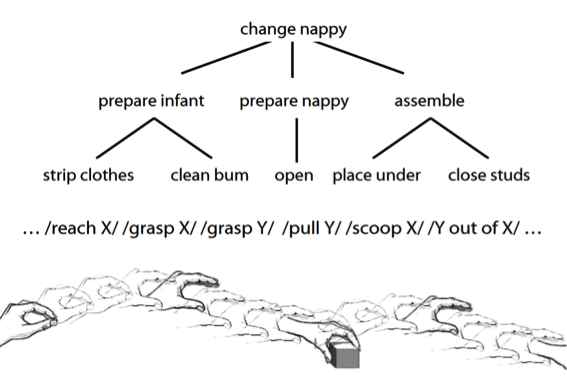
\includegraphics{figure_behaviour_reading.png}
\caption{
\label{figure:behaviour_reading}
	The structure of behaviour from bodily movement to plans. \citep[The lower image is adapted from][]{en_1462}.
}
\end{center}
\end{figure}

The challenge facing the mindreader is to recover some or all of this structure and the mental states which give rise to it by working backwards from the stream of bodily movement.  

The challenge facing a mindreader is a little bit like the challenge we face when we attempt to understand speech \citep{Baird:2001mb,Baldwin:2001rs}.%
\footnote{
	If the phonemic chunks are gestures, as some researchers suggest \citep[]{Browman:1992da, Liberman:2000gr}, then this view makes speech perception a special case of behaviour reading.}
[...]

Now in the case of speech recognition, no one supposes that we move from the acoustic signal to the intended message in a single step.
Rather, speech perception involves several stages: 
\begin{itemize}
\item 
segmenting continuous auditory and visual stimuli into phonemic chunks; 
\item 
assembling these chunks into word-sized units on the basis of sequential probabilities \citep[]{Saffran:1996aj}; 
\item 
recovering the meanings of individual words;
\item
 extracting clause- and sentence-sized complexes from these units on the basis of hierarchical patterns and prosodic cues \citep[]{Newport:2004wi, Soderstrom:2005zy}; 
\item
and so on.
\end{itemize}


Mindreading is surely also a process involving multiple steps.
We don't usually get from the bodily movements to the mental states in a single deft leap.
Rather there must be several intermediate processes.

I suggest that some of these intermediate processes are processes of pure goal ascription. 
Further, the basic units in terms of which mindreading proceeds---the equivalent of words---are already goal-directed actions.
Mindreading starts from behaviours which have already been identified as goal-directed actions.


\subsection{Multiple mechanisms for pure goal ascription}
Before we go on, note that it might be useful to have multiple mechanisms for goal ascription because performing actions involves multiple planning processes.
There is motor planning and there is practical reasoning.
Both result in goal-directed actions---reaching and grasping are goal directed actions---but probably involve quite different planning mechanisms.






\section{Obstacle to Pure Goal Ascription}
So far I've just been explaining why I'm excited about pure goal ascription, and why you should be too.

The question for this lecture is, 
\theQuestion

I want to start by introducing an apparent \textbf{obstacle} to the very possibility of pure goal ascription.

Earlier I said that \dfGoalAscription{}
Given this definition,
 goal ascription involves representing three things:
\begin{enumerate}
\item an action
\item an outcome
\end{enumerate}
and
\begin{enumerate}[resume]
\item the directedness of the action to the outcome.
\end{enumerate}
%
To anticipate, 
the obstacle to pure goal ascription will be that, apparently, representing the directedness of an action to an outcome involves representing mental states.
So pure goal ascription is impossible.

I think we can get around this obstacle.  
But let me go very slowly here and explain how the obstacle arises.
First it is important to see that the third item---representing the directedness---is necessary.

This is quite simple but very important, so let me slowly explain why goal ascription requires representing the directedness of an action to an outcome.
Imagine two people, Ayesha and Beatrice, who each intend to break an egg.
Acting on her intention, Ayesha breaks her egg.
But Beatrice accidentally drops her egg while carrying it to the kitchen.
So Ayesha and Beatrice perform visually similar actions which result in the same type of outcome, the breaking of an egg; 
	but Beatrice's action is not directed to the outcome of her action whereas Ayesha's is.
Goal ascription requires the ability to distinguish between Ayesha's action and Beatrice's action. 
This requires representing not only actions and outcomes but also the directedness of actions to outcomes.

This is why I say that goal ascription requires representing the directedness of an action to an outcome, and not just representing the action and the outcome.

\subsection{Directedness}
But what is it to represent the directedness of an action to an outcome?

Last week's lecture was all about the nature of this directedness. 
We asked, What is the relation between a purposive action and the outcome or outcomes to which it is directed?
We considered the standard view, on which this relation is explained in terms of an intention or other goal-representation.
We discussed two ways of understanding intention:
\begin{itemize}
\item as an action-causing belief--desire pair;
\end{itemize}
and, following Bratman,
\begin{itemize}
\item as an element in a planning process.
\end{itemize}
I suggested that we need both notions of intention.
But this week we can abstract from that debate and just think about intention as a mental state, remaining neutral on whether intention is somehow reducible to belief or desire or both.

If this were the whole truth about the directedness of actions to outcomes, then all goal ascription would involve representing mental states---in particular, intentions.
And pure goal ascription would be impossible.

\subsection{Teleological functions}
Can we understand directedness without intention?
One way to do this is to appeal to function.
Here is an example:
%
\begin{quote}
Atta ants cut leaves in order to fertilize their fungus crops (not to thatch the entrances to their homes) \citep{Schultz:1999ps}
\end{quote}
%
What does it mean to say that the ants’ grass cutting has this goal rather than some other? According to Wright:
\begin{quote}
`S does B for the sake of G iff: (i) B tends to bring about G; (ii) B occurs because (i.e. is brought about by the fact that) it tends to bring about G.' (Wright 1976: 39)
\end{quote}
%
For instance:
%
\begin{quote}
The Atta ant cuts leaves in order to fertilize iff: (i) cutting leaves tends to bring about fertilizing; (ii) cutting leaves occurs because it tends to bring about fertilizing.
\end{quote}
%
This has counterfactual consequences:
\begin{quote}
If S’s situation had differed such that B did not tend to bring about G, then B would not have occurred.
\end{quote}
%
In the simplest cases, (ii) is made true by history. In the past, behaviour like B occurred and brought about G. This B-like behaviour was then reproduced because it brought about G on that past occasion.

The readings for this lecture from Millikan explain how this idea can be developed in more sophisticated ways.
I don't want to get into the details.
What matters for present purposes is just that there are nonrepresentational ways of thinking about directedness.
That is, there are ways of thinking about directedness which don't involve thinking about intention or other representations.

I don't say that you can fully explain what it is for an action to be directed to an outcome without appeal to intention.
Surely you cannot.
The point is just that there are ways in which, however mistakenly, someone could represent directedness without representing intentions.

The point is this:
\begin{enumerate}
\item Goal ascription involves representing the directedness of an action to an outcome
\item If this directedness could be explained only in terms of intentions or other goal-representations, then pure goal ascription would be impossible because all goal ascription would involve representing representations.
\item But there is a way of understand directedness non-representationally, in terms of function.
\item And so it is possible that there are forms of goal ascription which do not involve representing mental states or any kind of representations.
\end{enumerate}
%
So there might be  \emph{pure} goal ascription, that is goal ascription which occurs independently of any knowledge of mental states.

So far I've been concerned with the very possibility of pure goal ascription.
We still have to answer the main question:
	\theQuestion


\section{Schematic answer}
Schematically we want to identify a relation, $R$, such that:
\begin{enumerate}
\item reliably $R(a,G)$ when and only when $a$ is directed\footnotemark to $G$; 
\item $R(a,G)$ is readily detectable; and 
\item $R(a,G)$ is readily detectable independently of any knowledge of mental states.
\end{enumerate}
%
\footnotetext{
We want this to be true whether $a$'s being directed to $G$ involves intention, function or motor representation.
}
%
We can make progress in explaining how pure goal ascription could work by identifying one or more values of $R$.
What could $R$ be?

\subsection{Define $R$ as teleological function}
Why not define $R$ in terms of teleological function?
This would enable us to meet the first condition but not the second.
How could we tell whether an action happens because it brought about a particular outcome in the past? 
This might be done with insects.
But it can's so easily be done with primates, who have a much broader repertoire of actions.

\subsection{Define $R$ as causation}
How about taking $R$ to be causation?
That is, how about defining $R(a,G)$ as $a$ causes $G$?
This proposal does not meet the first criterion, (1), above.
We can see this by mentioning two problems.

[*Might skip over-generate and discuss that as a problem for Rationality/Efficiency]
First problem: actions typically have side-effects which are not goals.
For example,
%---not a good example because can't be avoided by any account
%--- (would require attribution of desire)
%For example, walking to the corner results in me warming up, in me expending energy, and in me being at the corner.
%Sometimes I walk to the corner for exercise,
%so that being at the corner is an unwanted side-effect (I then have to walk back).
%And sometimes I walk to the corner to be at the corner (so that expending energy is an unwanted side-effect, I'd rather have been chauffeured there).  
suppose that I walk over here with the goal of being next to you.
This action has lots of side-effects: 
\begin{itemize}
\item 	I will be at this location.
\item	I will expend some energy.
\item	I will be further away from the front
\end{itemize}
These are all causal consequence of my action.
But they are not goals to which my action is directed.
So this version of $R$ will massively over-generate goals.

Second problem: actions can fail.  [...]
So this version of $R$ will under-generate goals.



\subsection{Define $R$ using the Principle of Rationality/Efficiency}
The leading candidate for $R$ is given in the Csibra and Gergeley's Principle of Rationality:
%
\begin{quote}
`an action can be explained by a goal state if, and only if, it is seen as the most justifiable action towards that goal state that is available within the constraints of reality' \citep[p.\ 255]{Csibra:1998cx} cf.\ \citep{Csibra:2003jv}.
\end{quote}
%
That is, we can define $R(a,G)$ as the relation which obtains when $a$ is `the most justifiable action towards' $G$ `that is available within the constraints of reality'.

A related but different `principle of efficiency' is:
%
\begin{quote}
`goal attribution requires that agents expend the least possible amount of energy within their motor constraints to achieve a certain end' \citep[p.\ 1061]{Southgate:2008el}.
\end{quote}
%
This principle suggests we might define $R(a,G)$ as the relation which obtains when $a$ is a means of achieving $G$ and any alternative available means would involve expending more energy.

In essence, the idea behind both principles is to identify $R$ with some kind of optimality.
In one case, optimality is explained in terms of rationality; in the other case optimality is understood as minimising energy.

How do these ideas stand up to our three criteria for $R$, (1)--(3) above?
I take it that they pass the third criterion (no reliance on knowledge of mental states).
And let's pass over whether rationality or energy expenditure is readily detectable for now; I don't think there are problems here.  

Focus on the first criterion, which we might loosely call \emph{reliability}. 
Roughly, the \emph{reliability} of a candidate for $R$ is the degree to which $R(a,G)$ corresponds to $G$ actually being a goal of $a$.

\subsubsection{First problem: side-effects}
A first problem is side-effects, which can be highly reliable.
Actions typically have side-effects which are not goals.
For example,
%---not a good example because can't be avoided by any account
%--- (would require attribution of desire)
%For example, walking to the corner results in me warming up, in me expending energy, and in me being at the corner.
%Sometimes I walk to the corner for exercise,
%so that being at the corner is an unwanted side-effect (I then have to walk back).
%And sometimes I walk to the corner to be at the corner (so that expending energy is an unwanted side-effect, I'd rather have been chauffeured there).  
suppose that I walk over here with the goal of being next to you.
This action has lots of side-effects: 
\begin{itemize}
\item 	I will be at this location.
\item	I will expend some energy.
\item	I will be this much further away from the front
\end{itemize}
These  are not goals to which my action is directed.
But they are things which my action would be a rational and efficient way of bring about.
So there is a risk that these optimising versions of $R$ will over-generate goals.

I think this first problem can be solved by introducing some additional constraints on $R$.
For instance, we can substantially mitigate the problem of side-effects by requiring that $R(a,G)$ hold only where $G$ is the type of outcome which is typically desirable for agents like $a$.


\subsubsection{Second problem: trade-offs}
One problem with defining $R$ in terms of minimising energy is that in acting we often face a trade off between how much energy to put into an action and how likely the action is to result in success.
Suppose I can save some energy by throwing the cup at the sink instead of walking over and carefully placing it in the sink,
and suppose that I choose to walk over and place the cup in the sink.
In this situation the principle of efficiency fails to identify $G$, placing the cup in the sink, as the goal of my action.
One way to address this problem might be to think of efficiency in terms of achieving a good trade-off between several factors:
not just energy but also the probability that a particular action will in fact result in the goal being achieved.


\subsubsection{Third problem: matching observer and agent}

A third potential problem concerning the reliability of both ideas, rationality and energy is even more obvious.
How good is the agent at optimising the rationality, or the efficiency, of her actions?
And how good is the observer at identifying the optimality of actions in relation to outcomes?
\textbf{
If there are too many discrepancies between
		how well the agent can optimise her actions
	and
		how well the observer can detect optimality,
then these principles will fail to be sufficiently reliable}.


\subsection{Summary so far}
The last two problems suggest that 
	we should not yet accept that appeal to the Principle of Rationality or of Efficiency will enable us how pure goal ascription might work.

I think we can make progress here by changing direction and thinking about motor planning.
This will initially seem unconnected;
I'll explain the connection at the end.


\section{Motor planning in action observation}

I want to approach this question directly by considering a puzzling findings:
motor planning occurs in action observation.
At least I think the findings should be puzzling.

*Start with a reminder about motor planning, illustrate with end-state optimality \citep{zhang:2007_planning}.
General idea is that planning can involve practical reasoning (explicit thinking) or motor processes.


\subsection{Motor planning occurs in action observation}
When observing an action,
	observers sometimes engage their own motor cognition 
	almost as if the observer were planning the agent's actions. 

To mention just one type of evidence for this claim,
observing actions sometimes facilitates performing compatible actions and interferes with performing incompatible actions, as several studies have shown \citep{brass:2000_compatibility, craighero:2002_hand, kilner:2003_interference, costantini:2012_does}. 
To give just one example, \citet{kilner:2003_interference} asked subjects to move their arms horizontally while they observed another person moving their arms either horizontally (that is, congruently) or vertically (that is, incongruently). 
They found that subjects' movements deviated significantly more when observing incongruent actions, and much as they would deviate if the subjects had been required to move their other arm incongruently. 
The effect cannot be explained as a consequence of observing mere movements because the same effect was not found when subjects observed a robot moving its arm.

Planning-like processes in action observation have also been demonstrated by measuring observers’ predictive gaze.  If you were to observe just the early phases of a grasping movement your eyes may jump to its likely target, ignoring nearby objects \citep{ambrosini:2011_grasping}. These proactive eye movements resemble those you would typically make if you were acting yourself \citep{Flanagan:2003lm}: in reaching for something, it is natural to look at the target rather than your hand.  Importantly, the occurrence of such proactive eye movements in action observation depends both on representing the outcome of an action (even temporary interference in the observer's ability to represent the outcome will interfere with the eye movements, \citealp{Costantini:2012fk}) and also on planning-like processes (requiring the observer to perform actions incongruent with those she is observing also interferes with proactive eye movements, \citealp{Costantini:2012uq}).  This, then, is further evidence that observers do something almost like planning the actions they observe.  

I think this should be puzzling.
Motor processes are for planning actions.
What are they doing in action observation?
Their presence becomes even more puzzling if we consider evidence that motor processes facilitate goal ascription.



\subsection{Motor processes facilitate goal ascription}
One source of evidence for the claim that motor representation can facilitate goal ascription involves motor expertise. 
If manipulating subjects' motor expertise can selectively affect their abilities to identify the goals of actions, this would be evidence that motor representation sometimes facilitates goal ascription.  Accordingly, \citet{casile:2006_nonvisual} asked subjects to make judgements about observed actions, including were some that are typically difficult to perform without training.  These actions were presented to subjects as point-light stimuli to ensure that only visual information about the actors' joint displacements was available.%
\footnote{
Readers who unfamiliar with point-light stimuli may view examples at http://www.biomotionlab.ca/Demos/BMLwalker.html.
The technique was introduced by \citet{johansson:1973_visual}.
}
They compared performance before and after subjects were trained to perform those actions themselves. They found that subjects' ability to accurately judge which action was being performed improved with the training. This is plausibly a consequence of increased motor expertise rather than any form of perceptual learning because the subjects were blindfolded during training (and the point-light stimuli on which their judgements were based are, of course, entirely visual). 

A related way to measure the effects of motor representation on judgements is to temporarily lesion part of the motor cortex using repetitive transcranial magnetic stimulation  (\citealp{urgesi:2007_representation, moro:2008_neural}).  \citet{urgesi:2007_representation} measured how long subjects took to make judgements about the type of action they were observing. They found that a temporary lesion to the premotor cortex, but not a temporary lesion to another brain area, increased the time taken to make action judgements. And the effect of lesioning the premotor cortex was specific to action judgements: subjects' abilities to make observational judgements identifying body parts was unaffected. Putting these studies together, we have evidence that enhancing motor representation (through training) sometimes facilitates judgements about the goals of actions, while destroying motor representation even temporarily can impair such judgements.

Further evidence comes from  studies of neurological deficits. If deficits in abilities to perform certain actions specifically impair abilities to make observational judgements about actions of that type, this would also indicate that motor representation can facilitate action judgements.  \citet{serino:2009_lesions_} compared the performances of control and hemiplegic subjects who were asked to identify actions. They found that ability to perform an observed action was correlated with ability to recognise that action. In particular, hemiplegic subjects were less accurate in identifying actions performed with limbs on the hemiplegic side of their bodies than actions performed with limbs on the unaffected side. By contrast, no such pattern was found for control subjects, which included both a group of healthy subjects and also a group of brain-damaged patients with no motor deficit.  (Including the latter group makes it possible to rule out the possibility that the findings were due to a general deficit in higher-order visual processing). 

Other evidence for a role for motor representation in judgements of action comes from research on apraxia. In one study subjects were asked to identify actions such as cutting paper and drinking with a straw on the basis of the sounds these actions produced. Subjects with limb apraxia showed an impairment in recognising hand-related actions (such as cutting paper) whereas subjects with buccofacial apraxia were impaired in recognising mouth-related actions (such as drinking); but no subjects showed a general impairment in recognising sounds and their significance \citep{pazzaglia:2008_sound_}. These links between motor deficits and action judgements provide further evidence that motor representation sometimes facilitates action judgements.%
\footnote{
In addition to facilitating judgements about the goals of observed actions, motor representations and processes may also sometimes facilitate judgements about the possibility of performing an action \citep{grosjean:2007_fitts_law, eskenazi:2009_role}.
}

Note that I am not suggesting that motor representation is \emph{necessary} for goal ascription.
This does not seem to be true.
As \citet{mahon:2008_action} notes, some studies suggest that apraxic subjects can recognise actions they cannot perform \citep[see also][]{hickok:2009_eight}. 
My claim is just that motor planning \emph{sometimes} facilitates goal ascription.
\textbf{Even if this facilitation were extremely rare phenomenon, we should still be puzzled as to how it could happen at all.}


\subsection{Summary so far}
This question is, \theQuestion 
I first considered whether we could answer this question by appeal to a Principle of Rationality or Efficiency.
We saw that this approach faces two problems.
Instead of trying to tackle those problems head-on, 
 I have only introduced a puzzle.
How could motor planning in action observation facilitate goal ascription?  
\newcommand{\thePuzzle}{How could motor planning in action observation facilitate goal ascription?  }
The  puzzle is, \thePuzzle 

Now I want to answer the question and resolve the puzzle with a single idea.
The idea is that% 
\newcommand{\theThesis}{planning abilities make pure goal ascription possible by enabling an observer to identify outcomes to which outcomes are directed. }
 \theThesis

\section{Planning as Goal Ascription}
I claim that \theThesis
How does this work?

Let us step back from motor phenomena to introduce the idea with an illustration.  
Observing Ayesha gathering some papers during a long meeting that shows no sign of ending, you conjecture that a goal of these and her next actions will be to leave discretely. You use this conjecture about the outcome to which Ayesha's actions are directed to determine one or more likely sequences of behaviours, almost as if you were planning from her point of view how to achieve that outcome. This leaves you with expectations concerning how she will act. You might be waiting for Ayesha, who has no other friends present, to give you a nod before quietly pushing away from the table. If what you observe matches these expectations, or if there are only deviations that can be explained in ways consistent with your conjecture about the goal of Ayesha's actions, then you may come to regard the conjecture as confirmed. But if there is a mismatch---if, for example, Ayesha signals that she wants attention and looks around to check people are looking at her---then you might reject the conjecture about the goal of her actions being to leave discretely. As this illustrates, determining how an action will or would unfold and then monitoring how it does unfold can ensure that there is a reliable connection between the action's being directed to a certain outcome and your representing that outcome. So the directedness of an action to a goal can be captured by a planning-like process together with appropriate monitoring.

In outline the link between an action and an outcome to which it is directed can be maintained like this. The representation of an outcome leads to a planning-like process which generates predictions about how the action will unfold, and this representation is weakened to the extent that the predictions are not met.  This is how planning processes can be co-opted to ensure that an outcome represented is likely to be an outcome to which the observed action is directed.

In effect, then,
	 motor planning can facilitate goal ascription
	 because it is used in order to apply something like the Principle of Rationality or Efficiency.



\section{Conclusion}
In this lecture I have been 
	pursuing a question about goal ascription 
and
	a puzzle about motor planning.
The question was, \theQuestion
The puzzle was, \thePuzzle

I think we can answer both by appeal to a simple thesis:
\begin{quote}
\theThesis
\end{quote}

This explains how motor planning in action observation might facilitate goal ascription: 
%it is being used to confirm or disconfirm conjectures about goals to which observed actions are directed.
Motor planning, like any planning process,  is sometimes useful for confirming or disconfirming conjectures about the outcomes to which actions are directed.
This is why it occurs in action observation and why it sometimes facilitates goal ascription.

I don't think that all pure goal ascription involves motor processes.
The idea is rather this.
Pure goal ascription involves planning-like processes, and motor processes are one suitable kind of planning-like process.
Another sort of planning process is practical reasoning, and we can use this for pure goal ascription too.

It is useful to have multiple mechanisms for goal ascription because performing actions involves multiple planning processes.


On The Question of how pure goal ascription could work,
	recall that we considered some problems for the idea that
	this could be explained by appeal to a Principle of Rationality or Efficiency.
The problems were:
%
\begin{itemize}
\item[2.] trade-offs---in essence, how to get the right principle
\item[3.] matching observer and agent---how to ensure a match between the agent's ability to plan optimally and the observers' ability to judge optimality
\end{itemize}
%
I think we can resolve both problems by thinking of the Teleological Stance not in terms of a specific principle, but in terms of planning.
\textbf{
The relation $R(a,G)$ should be defined relative to a planning mechanism.
For planning mechanism $M$, $R{_M}(a,G)$ holds just if $M$   were tasked with producing $G$ it would plan action $a$.}

With respect to the two problems:
 \begin{itemize}
\item[2.] trade-offs---we get the right principle by deferring to the kinds of planning mechanism responsible for producing the action.
\item[3.] matching observer and agent---we ensure a match insofar as observer an agent have similar planning mechanisms; this means, of course, that they must have similar expertise
\end{itemize}

So the question was, 
\theQuestion \\
Answer: we come up with conjectures about possible outcomes to which the actions are directed, then we generate predictions with a planning-like process.  Conjectures are confirmed to the extent that their  predictions match what is observed.

This simple idea allows us to finesse the Teleological Stance and, at the same time, to make sense of the fact that motor planning can facilitate goal ascription.


% --- OLD STUFF CUT ---
%\section{Segmentation}
%Think first about planning and performing an action.
%I intend to change the baby's nappy.
%I form three sub-plans: prepare baby, prepare nappy and assemble the two.
%[etc]
%
%Goal ascription involves starting from movements and recovering the structure.
%Two challenges.
%First is the segmentation challenge: to identify relevant units.
%Second is the outcome challenge: to identify outcomes to which the units are directed.
%
%
%[Point is to show it from the goal-ascriber's point of view.
%Can be agnostic about how segmentation works.
%Claim is just that there must be some process or other which segments actions.]
%
%But the constituents of actions are motor actions!
%So surely it makes sense to start with these?
%
%It may be important that we can represent others' actions motorically. 
%But the fact that we can do this does not show that we are engaged in goal ascription.
%It tells us that a certain format can be used in representing others' actions.
%It doesn't tell us \emph{how} we identify outcomes to which those actions are directed, however.
%
%
%Distinguish two claims:
%\begin{enumerate}
%\item The outcome is represented in a motor format
%\item The process of identifying the outcome is a motor process
%\end{enumerate}
%%
%At this point, the second claim should make no sense.
%\textbf{Motor processes are for planning actions.
%How could a motor process support goal ascription?}
%
%Evidence that it does: \citep{ambrosini:2011_grasping,ambrosini:2012_tie} \citep{costantini:2012_out} \citep{Costantini:2012fk}
%
%Capturing goals via a planning-like process ...
%
%This gives us one account of how pure goal ascription is possible: it is planning others actions.
%
%But it has various limits ...
%
%Note: don't necessarily have to think of it as specifically motor-planning.  Could be any kind of planning-like process.
%
%But when we generalise it in this way we move towards the Principle of Rationality or Efficiency, which is a further generalisation:
%\begin{quote}
%`an action can be explained by a goal state if, and only if, it is seen as the most justifiable action towards that goal state that is available within the constraints of reality' (Csibra and Gergely 1998: 255; cf. Csibra, Bíró, et al. 2003)
%\end{quote}
%%
%After all, how do we know what would be the most justifiable action towards a goal state?  
%We plan it!
%
%Limits ...
%
%
%Note: so far haven't distinguished heuristics from question about evidential basis.  (For this need to say that it's reasonable to trade on others planning as we do.)
%
%So how is pure goal ascription possible?
%By identifying maximally rational action:
%	which can be done by agent-neutral planning:
%	which can be implemented motorically.
%


\small
\bibliography{$HOME/endnote/phd_biblio}

\end{document}